\chapter{Testování}
%TODO vysledky zobrozene v TrackLabu !

%TODO mozna neco z testovani zaradit do sekce realizace. predevsim nejake promerovani parametru? a tady nechat jen zasadni info o dulezitych testech
\section{Napájení}
% TODO V2 uvest rozbehove sekvence celeho zarizeni  !!
% TODO V2 stailita 1V2ANA 1V2DIG pro Timepix2 !!
Na základní desce jsou generované celkem 3 napájecí úrovně z +5V externího napájení přes USB, jak bylo uvedeno v sekci \ref{napajeni}. A to napájecí úrovně +1.2 V, +2.5 V a +3.3 V. Zvlnění výstupního napětí bylo poté vždy měřeno na výstupu každého spínaného regulátoru se snahou vytvoření co nejkratší zemní smyčky mezi měřícím bodem a připojenou zemí osciloskopu. Měření nebylo ve všech případech s ohledem na velikost zemní smyčky ideální vzhledem k zapojení ve kterém je realizováno vyčítací rozhraní a to tedy v zapojení, kdy je deska s Timepix 2 nad základí deskou a tedy není možné se připojit sondou osciloskopu na vrchní stranu základní desky. I s ohledem na zmíněné problémy byly naměřeny tyto průběhy \ref{fig:napeti}. Kde CH3 je +2.5 V, CH2 +3.3V a CH1 poté +1.2 V.
\begin{figure}[h!]
	\centering
	\captionsetup{justification=centering}
	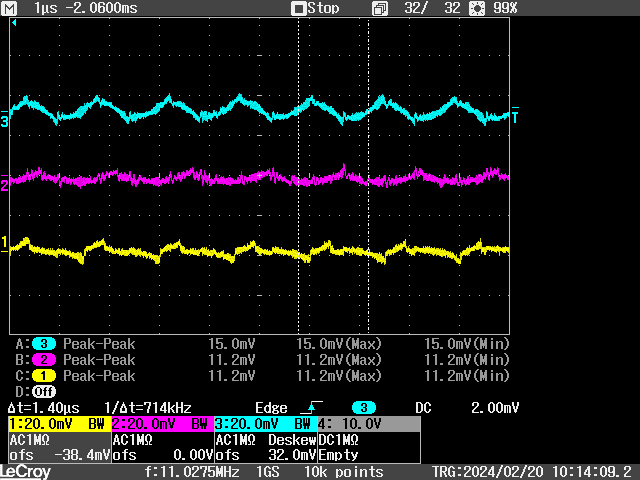
\includegraphics[scale=0.40]{./Mereni/ripple 3V3 - CH2 & 2V5 - CH3 & 1V2 - CH1, 2x 47uF.png}
	\caption{Zvlnění napětí výstupních napětí +2.5V, +3.3 V a +1.2 V } 
	\label{fig:napeti}
\end{figure}
Stabilní stejnosměrné hodnoty výše uvedených napájecích úrovní je možné vidět na obrázku 
\begin{figure}[h!]
	\centering
	\captionsetup{justification=centering}
	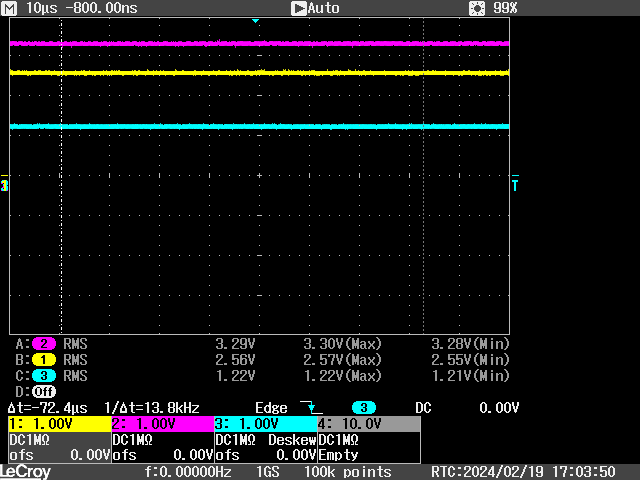
\includegraphics[scale=0.40]{./Mereni/vout 3V3 & 2V5 & 1V2.png}
	\caption{Stjenosměrné úrovně výstupních napětí spínaných regulátorů na základní desce \ref{zakladni deska}} 
	\label{fig:urovne}
\end{figure}

%todo ripple output of HV?
\section{Vysokonapěťový zdroj}
% Nastaveni VN zdroje
Zapojení vyskonapěťového zdroje a princip měření vysokého napětí, které se generuje na desce s Timepix 2 \ref{Deska s Timepix2} je popsán v části textu \ref{VN zdroj}. Velikost vysokého napětí je nastavována pomocí 8 bitového čísla. Závislost 8 bitové hodnoty na výstupním napětí vysokonapěťového zdroje je možné vidět na obrázku \ref{fig:hv_hex}.
\begin{figure}[h!]
	\centering
	\captionsetup{justification=centering}
	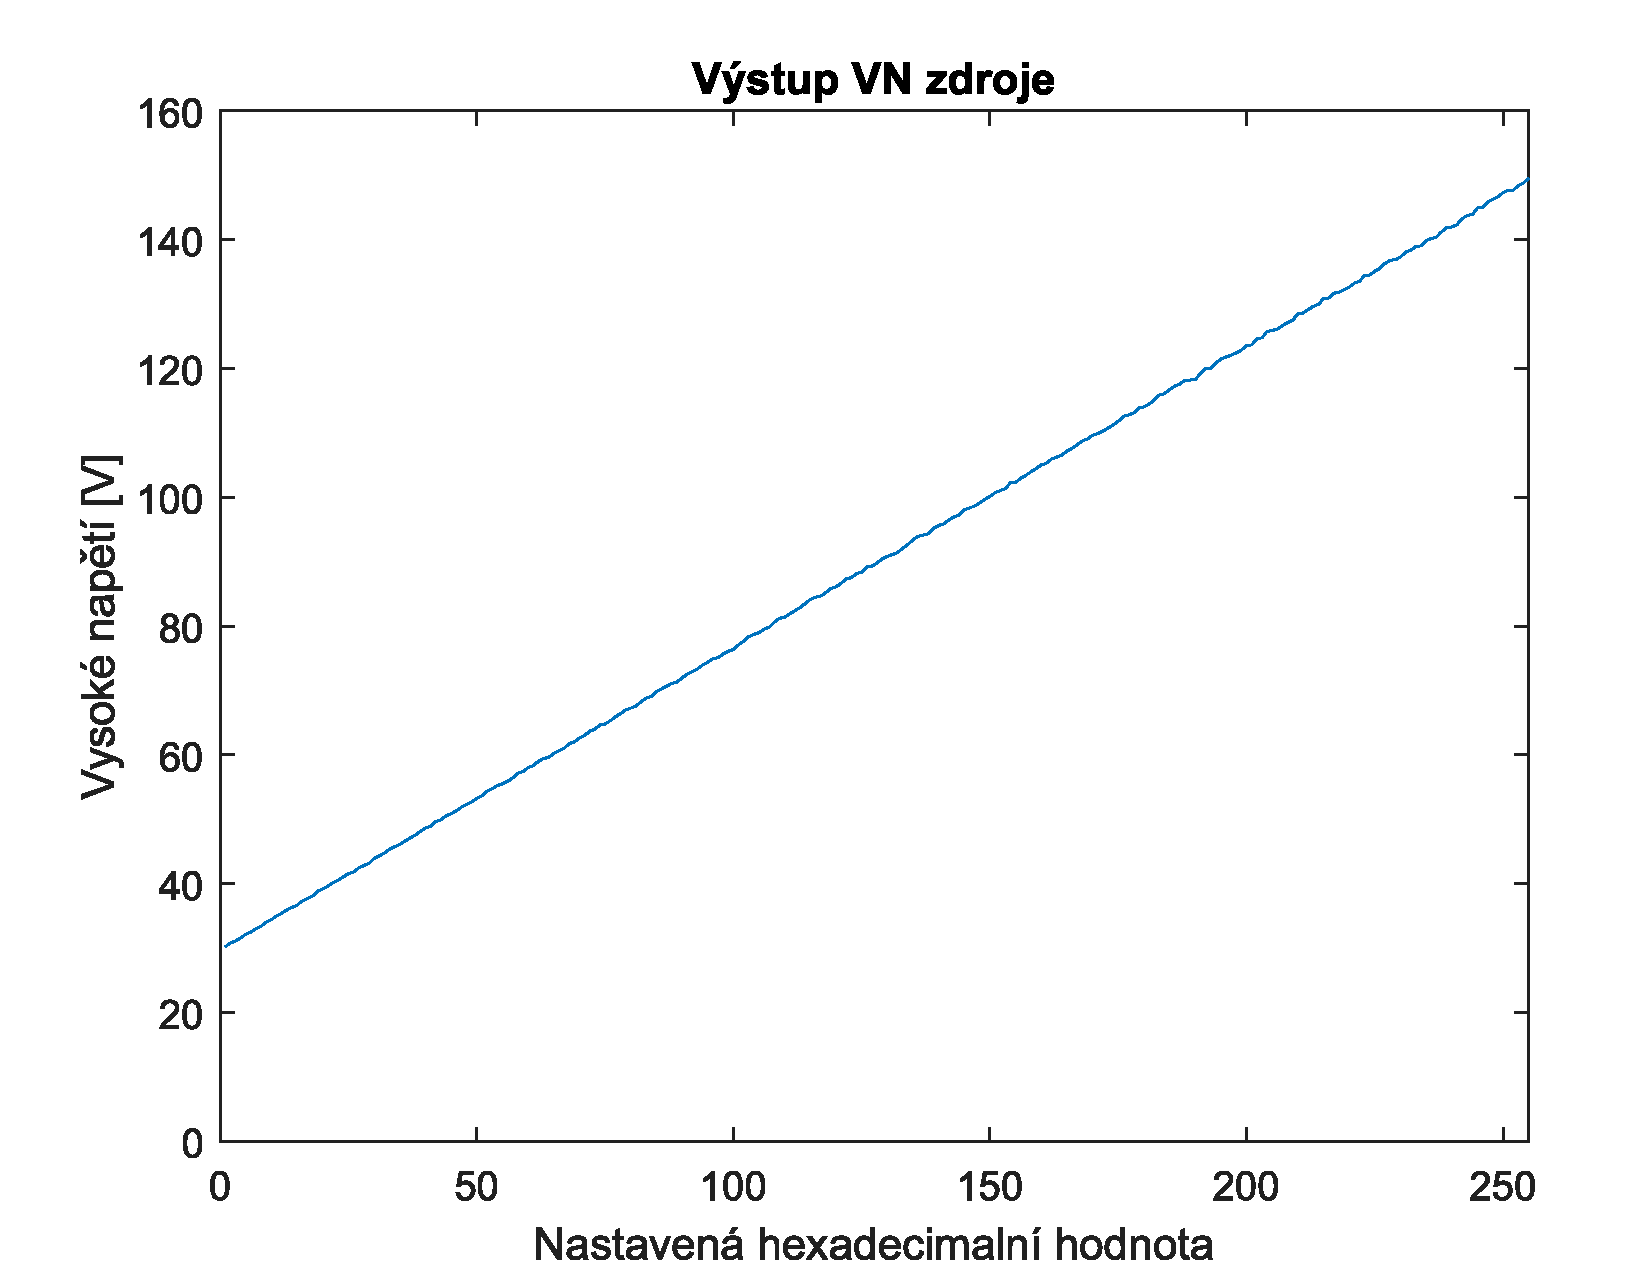
\includegraphics[scale=0.40]{./Mereni/hv_hex_small.pdf}
	\caption{Závislost vstupní 8 bitové hodnoty na výstupním napětí VN zdroje} 
	\label{fig:hv_hex}
\end{figure}
 
\section{Měření teploty}
V této práci bylo implementováno měření teploty pomocí externího teplotního senzoru na desce s detektorem Timepix 2 \ref{Deska s Timepix2} a měření teploty za využití interního měření teploty detektoru Timepix 2.
% TODO výpis z Terminalu, jeste lepe z TrackLabu
% TODO promereni teploty s mechanikou ??
\subsection{Měření teploty vyčítacího rozhraní}
Typ senzoru který byl pro tuto práci vybrán pro měření teploty na desce s Timepix 2 byl podrobně popsán v části \ref{Mereni teploty}. Pokud dojde k uživatelskému příkazu, který požaduje informaci o teplotě, následuje proces vyčtení teploty ze senzoru, který je zjednodušeně popsán diagramem na obrázku \ref{fig:diagram}.
\begin{figure}[h!]
	\centering
	\captionsetup{justification=centering}
	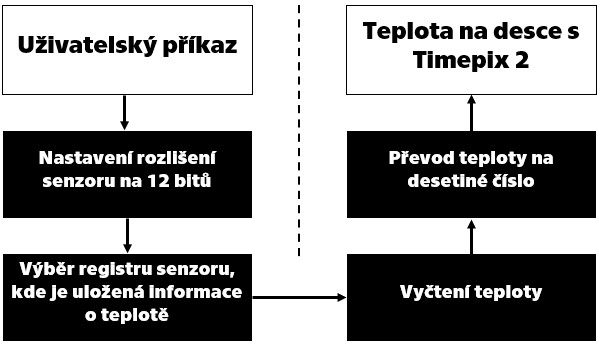
\includegraphics[scale=0.50]{teplota diagram.jpg}
	\caption{Diagram průběhu vyčtení teploty ze senzoru TMP 100 na desce s Timepix 2} 
	\label{fig:diagram}
\end{figure}

\subsection{Měření teploty Timepix2}
Pixelový detektor Timepix 2 umožnuje monitorovat vnitřní teplotu detektoru. Hodnota výsledné teploty detektoru je poté dle simulace teploty detektoru v závislosti na napěťové referenci popsána na obrázku \ref{fig:tpx2_temp}. Pro získání teploty detektoru je zapotřebí naměření dvou analogových hodnot z obrázku \ref{fig:tpx2_temp} označovaných jako Vtemp a Vbg. Pro získání těchto analogových hodnot je nejprve zapotřebí nastavit, jaká hodnota analogového napětí bude na výstupu pinu Timepix 2 označovaného jako DACOUT. Výstup DACOUT Timepix 2 je poté zpracován interním ADC převodníkem mikroprocesoru na základní desce \ref{zakladni deska}. Příklad výběru hodnoty na výstup DACOUT detektoru Timepix 2 a převod získaných hodnot na odpovídající teplotu lze vidět v \ref{kod_temp_tpx2}.
\begin{lstlisting}[frame=single, language=C, caption={Výběr výstupu DACOUT detektoru Timepix2 a odečtení hodnoty detektoru}, label=kod_temp_tpx2]
// GET DAC : VBG_TEMP
uint8_t set_dacoutsel[0] = VBG_TEMP; 
float vtemp = 0;
// set what type of DAC will be on DACOUT output								   
if(tpx2_set_reg_8b(TPXA, SET_DACOUTSEL, set_dacoutsel) != TPX_OK) {    
	Error_Handler();
}
if(board_tpx2_get_dacout(TPXA, &vtemp) != BOARD_OK) {
	Error_Handler();
}
// Sim. -> TT. // Temp. into real value in ^C.
float tpx2_temp = 471.99*(vtemp - vbg)/1000 - 179.14;					
\end{lstlisting}

\begin{figure}[h!]
	\centering
	\captionsetup{justification=centering}
	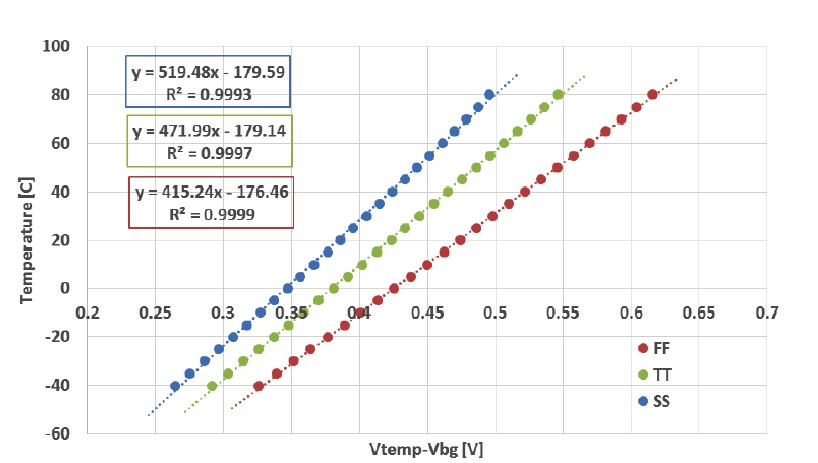
\includegraphics[scale=0.50]{tpx2_temp.jpg}
	\caption{Simulace teploty detektoru Timepix2 v závisloti na hodnotě napěťové reference \cite{tpx2_manual}.} 
	\label{fig:tpx2_temp}
\end{figure}



\section{Komunikační rozhraní s Timepix 2}		% promřování logických urovni komunkikace, rychlosti atd..
%todo logicke urovne SLVS, rychlosti komunikace -> need V2. MCLOCK..
Komunikační rozhraní detektoru Timepix 2 bylo popsáno v části textu \ref{Komunikacni rozhrani}. Následná  realizace komunikace s Timepix 2 pak v části \ref{CPLD konverze}. K měření diferenciálních komunikačních signálů byla použita aktivní diferenciální sonda s osciloskopem. Měření probíhalo při frekvenci komunikace 20 Mhz. Na obrázku \ref{fig:MCLOCK_DIFF_PROBE} můžete vidět průběh komunikačních hodin. Konkrétně CH 2 z obrázku \ref{fig:MCLOCK_DIFF_PROBE} je výstup hodinového signálu SPI komunikace. Kanál CH 1 je poté naměřený diferenciální signál aktivní diferenciální sondou po konverzi logické úrovně v CPLD. Jak je vidět parametry diferenciálního signálu odpovídají parametrů SLVS komunikace. 
\begin{figure}[h!]
	\centering
	\captionsetup{justification=centering}
	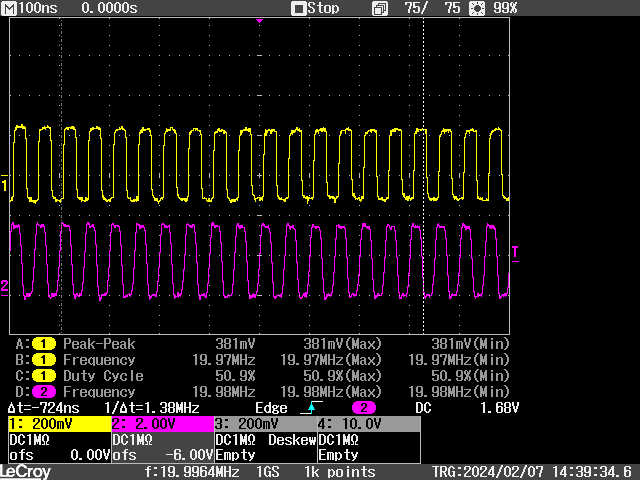
\includegraphics[scale=0.40]{./Mereni/MCLOCK_DIFF_PROBE.png}
	\caption{Průběh hodinového signálu pro komunikaci s Timepix 2} 
	\label{fig:MCLOCK_DIFF_PROBE}
\end{figure}

\section{Digitální test Timepix 2} %popis prubehu a vysledku
Funkčnost komunikace s detektorem Timepix 2 byla ověřena pomocí digitálních testů, jednotlivé testy budou popsány v následujících částech.
	\subsection{Vyčtení chip ID}
	Prvním digtálním testem, který byl implementován byl test, který vyčítá sériové výrobní číslo, označované jako CHIP ID, které je pro každý detektor Timepix 2 jedinečné a předem známé. Pro správné vyčtení CHIP ID detektoru je nejprve zapotřebí přivést napájecí napětí +2.5 V na pin VDD33, jak bylo popsáno v části \ref{Technicka specifikace}. Hodnota CHIP ID je poté uložena v 32-bitové registru Timepix 2. Vyčtením tohoto registru dostáváme 32 bitovou hodnotu, kterou pomocí známé transformace převedeme na skutečnou hodnotu CHIP ID, která odpovídá předem známé hodnotě, jež je dodávaná přímo při dodání detektoru Timepix 2.
	%TODO hodnota CHIP ID
	\subsection{Vyčtení a zapsání pixelových matic}
	Pomocí výše uvedeného testu, vyčtení CHIP ID detektoru došlo k otestování vyčítaní základních registrů detektoru Timepix 2. Dalším digitálním testem je poté zápis a vyčtení všech čítačů, používajících se na měření. Popis čítačů Timepix 2, lze najít v části \ref{Digitálni cast}.
	\par Zápis do digitálních čítačů slouží jen pro digitální testování, při samotném měření se tato funkce nevyužívá. Celkem při tomto digitálním testu dojde k zápisu hodnot do všech čtyřech dostupných čítačů Timepix 2 a následnému vyčtení. Celkem je zapsáno 5 testujících obrazů. Zapsané obrazce byly zvoleny viz. tabulka \ref{tab:obraz} Při tomto digitálním dochází k zápisu 327 680B dat a jejich opětovnému vyčtení. Digi
	\begin{table}[h!]
		\centering
		\begin{tabular}{ |P{3cm}|P{3cm}|  }
			\hline
			\multicolumn{2}{|c|}{Vybrané zapsané obrazce} \\
			\hline
			Test  & Obraz\\ \hline \hline 
			1 & 0xFF \\ \hline 	
			2 & 0x00 \\ \hline 		 
			3 & INC \\ \hline
			4 & DEC \\ \hline
			5 & 0xAA\\ \hline
		\end{tabular}
		\caption{Digitální test, zapisované hodnoty}
		\label{tab:obraz}
	\end{table}
\section{USB komunikace}s
%todo, dokumentace funkčnosti... -> VCM, pak UDP pres USB

\section{Měření spotřeby}
%todo spotreba, bez chipu, s chipem, zavislosti?
	\subsection{Porovnání spotřeby} % TODO nebo jen uvest parametry?
	
\section{Dosažené parametry}
% TODO shrnuti nosazenych parametru namerenych vyse